%%
%% This is file `sample-sigconf-authordraft.tex',
%% generated with the docstrip utility.
%%
%% The original source files were:
%%
%% samples.dtx  (with options: `all,proceedings,bibtex,authordraft')
%% 
%% IMPORTANT NOTICE:
%% 
%% For the copyright see the source file.
%% 
%% Any modified versions of this file must be renamed
%% with new filenames distinct from sample-sigconf-authordraft.tex.
%% 
%% For distribution of the original source see the terms
%% for copying and modification in the file samples.dtx.
%% 
%% This generated file may be distributed as long as the
%% original source files, as listed above, are part of the
%% same distribution. (The sources need not necessarily be
%% in the same archive or directory.)
%%
%%
%% Commands for TeXCount
%TC:macro \cite [option:text,text]
%TC:macro \citep [option:text,text]
%TC:macro \citet [option:text,text]
%TC:envir table 0 1
%TC:envir table* 0 1
%TC:envir tabular [ignore] word
%TC:envir displaymath 0 word
%TC:envir math 0 word
%TC:envir comment 0 0
%%
%% The first command in your LaTeX source must be the \documentclass
%% command.
%%
%% For submission and review of your manuscript please change the
%% command to \documentclass[manuscript, screen, review]{acmart}.
%%
%% When submitting camera ready or to TAPS, please change the command
%% to \documentclass[sigconf]{acmart} or whichever template is required
%% for your publication.
%%
%%
\documentclass[acmsmall,screen,review,anonymous]{acmart} % FSE review version
%%
%% \BibTeX command to typeset BibTeX logo in the docs
\AtBeginDocument{%
  \providecommand\BibTeX{{%
    Bib\TeX}}}

%% Rights management information.  This information is sent to you
%% when you complete the rights form.  These commands have SAMPLE
%% values in them; it is your responsibility as an author to replace
%% the commands and values with those provided to you when you
%% complete the rights form.
\setcopyright{acmlicensed}
\copyrightyear{2026}
\acmYear{2026}
\acmDOI{XXXXXXX.XXXXXXX}
%% These commands are for a PROCEEDINGS abstract or paper.
\acmConference[Conference ICSE '2026]{IEEE/ACM International Conference on Software Engineering}{April 12--18,
  2026}{Rio de Janeiro, Brazil}
%%
%%  Uncomment \acmBooktitle if the title of the proceedings is different
%%  from ``Proceedings of ...''!
%%
%%\acmBooktitle{Woodstock '18: ACM Symposium on Neural Gaze Detection,
%%  June 03--05, 2018, Woodstock, NY}
\acmISBN{978-1-4503-XXXX-X/2018/06}


\usepackage{listings}
\usepackage{algorithm}
\usepackage{algorithmic}
% \usepackage{algorithmicx}
% \usepackage{algpseudocode}
% \usepackage{algorithm2e}

\renewcommand{\algorithmicrequire}{\textbf{Input:}}
\renewcommand{\algorithmicensure}{\textbf{Output:}}

% \algnewcommand\algorithmicforeach{\textbf{for each}}
% \algdef{S}[FOR]{ForEach}[1]{\algorithmicforeach\ #1\ \algorithmicdo}

%%
%% Submission ID.
%% Use this when submitting an article to a sponsored event. You'll
%% receive a unique submission ID from the organizers
%% of the event, and this ID should be used as the parameter to this command.
%%\acmSubmissionID{123-A56-BU3}

%%
%% For managing citations, it is recommended to use bibliography
%% files in BibTeX format.
%%
%% You can then either use BibTeX with the ACM-Reference-Format style,
%% or BibLaTeX with the acmnumeric or acmauthoryear sytles, that include
%% support for advanced citation of software artefact from the
%% biblatex-software package, also separately available on CTAN.
%%
%% Look at the sample-*-biblatex.tex files for templates showcasing
%% the biblatex styles.
%%

%%
%% The majority of ACM publications use numbered citations and
%% references.  The command \citestyle{authoryear} switches to the
%% "author year" style.
%%
%% If you are preparing content for an event
%% sponsored by ACM SIGGRAPH, you must use the "author year" style of
%% citations and references.
%% Uncommenting
%% the next command will enable that style.
%%\citestyle{acmauthoryear}


%%
%% end of the preamble, start of the body of the document source.
\begin{document}

\newcommand{\circlenum}[1]{\normalsize{\textcircled{\scriptsize{\emph{#1}}}}\normalsize}

%%
%% The "title" command has an optional parameter,
%% allowing the author to define a "short title" to be used in page headers.
\title{Toward Semantic Understanding of Stripped Binary Android Native Libraries: A framework Based on Multi-Agent System}

%%
%% The "author" command and its associated commands are used to define
%% the authors and their affiliations.
%% Of note is the shared affiliation of the first two authors, and the
%% "authornote" and "authornotemark" commands
%% used to denote shared contribution to the research.
\author{Ben Trovato}
\authornote{Both authors contributed equally to this research.}
\email{trovato@corporation.com}
\orcid{1234-5678-9012}
\author{G.K.M. Tobin}
\authornotemark[1]
\email{webmaster@marysville-ohio.com}
\affiliation{%
  \institution{Institute for Clarity in Documentation}
  \city{Dublin}
  \state{Ohio}
  \country{USA}
}

\author{Lars Th{\o}rv{\"a}ld}
\affiliation{%
  \institution{The Th{\o}rv{\"a}ld Group}
  \city{Hekla}
  \country{Iceland}}
\email{larst@affiliation.org}

\author{Valerie B\'eranger}
\affiliation{%
  \institution{Inria Paris-Rocquencourt}
  \city{Rocquencourt}
  \country{France}
}

\author{Aparna Patel}
\affiliation{%
 \institution{Rajiv Gandhi University}
 \city{Doimukh}
 \state{Arunachal Pradesh}
 \country{India}}

\author{Huifen Chan}
\affiliation{%
  \institution{Tsinghua University}
  \city{Haidian Qu}
  \state{Beijing Shi}
  \country{China}}

\author{Charles Palmer}
\affiliation{%
  \institution{Palmer Research Laboratories}
  \city{San Antonio}
  \state{Texas}
  \country{USA}}
\email{cpalmer@prl.com}

\author{John Smith}
\affiliation{%
  \institution{The Th{\o}rv{\"a}ld Group}
  \city{Hekla}
  \country{Iceland}}
\email{jsmith@affiliation.org}

\author{Julius P. Kumquat}
\affiliation{%
  \institution{The Kumquat Consortium}
  \city{New York}
  \country{USA}}
\email{jpkumquat@consortium.net}

%%
%% By default, the full list of authors will be used in the page
%% headers. Often, this list is too long, and will overlap
%% other information printed in the page headers. This command allows
%% the author to define a more concise list
%% of authors' names for this purpose.
\renewcommand{\shortauthors}{Trovato et al.}

%%
%% The abstract is a short summary of the work to be presented in the
%% article.
\begin{abstract}
  An increasing number of Android applications encapsulate parts of their logic in native code to improve execution efficiency or to impede reverse engineering. Ultimately, the native code is compiled into binaries, specifically shared objects designated by the .so suffix. Despite extensive research on stripped binaries, there remains a significant gap in the detailed exploration of those on the ARM64 architecture, particularly for Android Native Libraries. This paper proposes a framework based on a Multi-Agent System that models the manual reverse engineering process. This framework integrates three key components: Ghidra for static analysis (providing assembly and pseudo-C code), Frida Stalker for dynamic analysis (simulating debugging behaviors), and a Large Language Model (LLM) for automated test case generation. To evaluate our method's effectiveness, we constructed a new dataset of stripped ARM64 binaries by collecting open-source Android applications with native libraries from GitHub. Extensive experiments demonstrate that our method has achieved state-of-the-art (SOTA) performance in semantic understanding tasks, including function name recovery and comment generation.
\end{abstract}

%%
%% The code below is generated by the tool at http://dl.acm.org/ccs.cfm.
%% Please copy and paste the code instead of the example below.
%%
\begin{CCSXML}
<ccs2012>
 <concept>
  <concept_id>00000000.0000000.0000000</concept_id>
  <concept_desc>Do Not Use This Code, Generate the Correct Terms for Your Paper</concept_desc>
  <concept_significance>500</concept_significance>
 </concept>
 <concept>
  <concept_id>00000000.00000000.00000000</concept_id>
  <concept_desc>Do Not Use This Code, Generate the Correct Terms for Your Paper</concept_desc>
  <concept_significance>300</concept_significance>
 </concept>
 <concept>
  <concept_id>00000000.00000000.00000000</concept_id>
  <concept_desc>Do Not Use This Code, Generate the Correct Terms for Your Paper</concept_desc>
  <concept_significance>100</concept_significance>
 </concept>
 <concept>
  <concept_id>00000000.00000000.00000000</concept_id>
  <concept_desc>Do Not Use This Code, Generate the Correct Terms for Your Paper</concept_desc>
  <concept_significance>100</concept_significance>
 </concept>
</ccs2012>
\end{CCSXML}



%%
%% Keywords. The author(s) should pick words that accurately describe
%% the work being presented. Separate the keywords with commas.
\keywords{Do, Not, Us, This, Code, Put, the, Correct, Terms, for,
  Your, Paper}
%% A "teaser" image appears between the author and affiliation
%% information and the body of the document, and typically spans the
%% page.
% \begin{teaserfigure}
%   \includegraphics[width=\textwidth]{sampleteaser}
%   \caption{Seattle Mariners at Spring Training, 2010.}
%   \Description{Enjoying the baseball game from the third-base
%   seats. Ichiro Suzuki preparing to bat.}
%   \label{fig:teaser}
% \end{teaserfigure}

\received{20 February 2007}
\received[revised]{12 March 2009}
\received[accepted]{5 June 2009}

%%
%% This command processes the author and affiliation and title
%% information and builds the first part of the formatted document.
\maketitle


\section{Introduction}



\section{Background and Motivation}



\subsection{Challenges}
Although the task of recovery of binary function names has garnered significant attention, leading to a variety of methods that leverage different information in different ways and have each achieved a certain degree of success, we have identified three persistent challenges in this domain.

\textbf{C1: Generalizability of Function Name Recovery}. Previous research has predominantly framed binary function name recovery as a classification task (e.g., XFL, AsmDepictor, SymLM). This approach presupposes that the target function names, or at least parts of them, exist within their predefined set of classes. However, such an assumption often does not hold in real-world scenarios. Although various techniques have been employed to mitigate the Out-of-Vocabulary (OOV) problem, it remains an unavoidable issue, particularly when these methods are applied to novel datasets. The recent state-of-the-art technique, SymGen, reformulates the task as a generation problem, fundamentally resolving the OOV issue by fine-tuning a Large Language Model (LLM). Nevertheless, due to resource and dataset constraints, such generative approaches typically resort to fine-tuning smaller models (e.g., CodeLlama-34B). This reliance on smaller models significantly curtails their effectiveness when the target function or its other architectural variants are not present in the fine-tuning data. The core reason is the limited capacity of smaller models to truly comprehend the semantics of binary code, which hinders their ability to generalize to unseen functions. Furthermore, the ever-increasing volume of binary code in modern software poses an additional threat to the generalizability of the strategy of fine-tuning LLM.

\textbf{C2: Pervasive Function Calls}. Complex function call graphs are an ubiquitous feature of code written by developers. Figure xxx shows the function \lstinline{copynode234}, which employs recursion to traverse a 2-3-4 tree while delegating the node copying task to the \lstinline{copyfn} function. Although some small functions may be inlined by the compiler, the vast majority of intricate call relationships are preserved in binaries. At the source code level, one can often infer the semantics of a function by examining the names of the functions it calls. In stripped binaries, however, this semantic information is largely lost, leaving us with only the starting addresses of callee functions (e.g., \lstinline{FUN_00123456}), which substantially complicates semantic comprehension. A more formidable challenge arises from the widespread use of indirect calls in C/C++ (e.g., function pointers, virtual function tables), which makes it impossible to resolve call targets through static analysis alone. \lstinline{FUN_00125a60} in Figure xxx is the decompiled counterpart of copynode234. The call to the copyfn function corresponds to \lstinline{(*param_2)(param_3)} on line 5. Since the target of this call depends on the value of \lstinline{param_2}, its actual destination cannot be determined by purely static analysis. This ambiguity obstructs the understanding of the callee's semantics, impeding the recovery of \lstinline{FUN_00125a60}.

Taking SymGen as an example, we observed that many of its predicted names were placeholders like \lstinline{FUN_xxxxxx}. A closer analysis revealed that this often occurs when the primary logic of a target function A is implemented by calling another function B. Because B's name has been stripped and replaced with a placeholder, the predicted name for A inherits this placeholder. While some methods like SymLM and NERO have attempted to model call context information, their performance has been suboptimal. We argue that this is primarily because they fail to account for the topological dependency in the call graph; that is, the logic of copynode234 can be accurately inferred only after the logic of copyfn has been determined.

\textbf{C3: Unpredictable Execution Behavior}. We contend that static code analysis alone is insufficient for a complete understanding of program logic, especially when the code involves dynamic behaviors influenced by runtime parameters or external environment variables. This holds true even for source-level code comprehension, although the rich semantic information available in source code often mitigates its impact. In the context of stripped binaries, the effect of dynamic behavior becomes far more pronounced. This challenge is further exacerbated by modern compilers, which extensively employ optimization techniques that obscure the code's true behavior, making it exceedingly difficult to grasp its logic from a static view.

Consider a function \lstinline{ParseNanos} from a real-world project (RTranslator) and its decompiled variant, shown in Figures xxx and xxx, respectively. The function accepts string pointer data, writes the parsed nanosecond value to the output parameter \lstinline{nanos}, and returns the new position of the data pointer. Its core logic, a loop spanning lines 4-8, extracts digits from the string and stores them in value. Lines 9-12 pad the number with zeros if it has fewer than 9 digits, and the final result is output on lines 13 and 14. The source code is readily understandable. However, after compilation with optimizations (-O2), its decompiled representation exhibits altered logical expressions, although the functionality remains equivalent. For example, the original condition "parse at most 9 characters" is transformed into \lstinline{if(8 < uVar3)}. As shown in Table xxx, this transformation not only increases the difficulty of semantic understanding but can also mislead predictions of models.

\subsection{Motivation}

In recent years, LLMs have demonstrated remarkable efficacy across numerous source-level programming tasks. Pioneering research such as SymGen and FoC has illuminated their potential for understanding the semantics of binary code. We are therefore convinced that leveraging capacities of LLMs remains a promising strategy. To address challenge \textbf{C1}, instead of fine-tuning small models like CodeLlama, our approach, HyBinMAS, utilizes a larger, general-purpose LLM as its foundational component, structured within a Multi-Agent System. It eliminates the need for meticulous fine-tuning, thereby attaining superior generalizability, considering the inherent drawbacks of fine-tuning large-scale LLMs, which is both resource-intensive and time-consuming.

To tackle \textbf{C2}, HyBinMAS begins by preprocessing the target binary file, employing a hybrid static-dynamic analysis to resolve function call graphs. It then explicitly considers these call relationships during the name prediction phase. We observed that reverse engineers often adopt a recursive mindset when analyzing function calls: if function A calls function B, they typically analyze B first and use the resulting semantic understanding to inform their analysis of A. Inspired by this practice, HyBinMAS follows a similar bottom-up process. It first recovers the names of the functions called within a target function and then leverages this information to recover the name of the target function itself. Returning to the example in Figure xxx, by analyzing the call relationships of \lstinline{FUN_00125a60}, we can determine the actual function pointed to by \lstinline{param_2}, deduce that its logic is related to copying, and consequently predict a more accurate name, as shown in Figure xxx. Without this strategy, one might only discern that the function performs a recursive traversal, without knowing the specific operation being performed during the traversal.

 An experienced reverse engineer not only "reads" the code but also "runs" it. After forming an initial hypothesis about the code's semantics through static inspection, they will construct test cases to execute the function and observe its dynamic behavior. This allows them to validate or refute their initial assumptions and guide further analysis. We believe this is a highly effective method for addressing the challenge of \textbf{C3}. For the function \lstinline{ParseNanos}, the initial LLM predictions in Table xxx were semantically close but incorrect regarding the precise number of digits, which is a fitting example of being misled by compilation optimizations. Based on the initial semantic hypothesis, HyBinMAS generates the test cases shown in Table xxx. Upon execution, it observes that for test case 4, which expects only the first 8 characters to be parsed, all 9 digits are actually processed. This execution trace is summarized into a feedback report that directs the LLM to revise its previous inference. Through several iterations of this process, HyBinMAS arrives at the more accurate semantic prediction shown in the HyBinMAS column of Table xxx.

Furthermore, we acknowledge that not all functions can be executed successfully. A more complex example is presented in Figure xxx (see Appendix for decompiled code). The LLM's initial semantic interpretation was simply \lstinline{remove}, a description that is clearly imprecise. However, because this function takes a pointer to a custom structure as a parameter, attempts to generate test cases and execute it frequently lead to illegal memory access and program crashes. HyBinMAS addresses this by using an additional LLM to summarize the generated test cases and the execution failure logs into a new feedback report. By providing this consolidated feedback to the primary LLM, HyBinMAS facilitates a more accurate prediction: \lstinline{remove_env}.


% ### Challenges

% 虽然二进制函数名恢复任务广受关注,在该领域涌现了许多相关的方法(综述中提到的方法),它们采用不同方式利用不同的信息并分别取得了一定程度的进展。但是我们发现二进制函数名称恢复任务仍然存在如下3个挑战:

% #### C1 方法的泛用性

% 以往的研究都将二进制函数名称恢复任务建模为一个分类任务(XFL、AsmDepictor、SymLM),这意味着它们的方法建立在目标函数名(部分)存在于它们的类别集合中。但是这样的假设往往很难在现实的函数名称恢复任务中成立,虽然它们采用了不同方式缓解OOV的问题,但OOV问题仍然不可避免,特别是当被用到新数据集中时。最近的SOTA(SymGen)将函数名称恢复任务建模为一个生成任务并通过微调一个LLM来处理,并从根本上解决了OOV的问题。但是由于资源和数据集的限制,这一类方法通常选择参数量较小的模型(例如CodeLLama-34B)进行微调,这使得被预测的函数或其指定架构的变体不在微调数据集中时,方法的有效性大打折扣,这主要是因为小参数模型难以真正理解二进制代码的知识,因而难以完全将其推广到未见过的二进制函数中。而且如今日益增多的二进制代码也使得微调LLM的策略的泛用性受到一定程度的影响。

% #### C2 广泛存在的函数调用

% 现实中的程序员编写的代码中广泛存在复杂的函数调用情况,如图xxx所示,函数copynode234内部通过调用copyfn完成实际的节点复制功能,并通过递归调用自身完成遍历2-3-4树的操作。虽然在将源码编译成二进制代码时,有些短小的函数会发生函数内联,但是绝大多数的复杂的调用关系仍然会被保留下来。对于源码级的函数语义理解任务,可以通过观察被调用函数的函数名来推测其语义,但在stripped binaries中,我们丢失了绝大多数的语义信息,我们只能知道被调用函数的起始地址(例如FUN_00123456),这无疑加剧了函数理解的困难。更困难的是,C/C++代码中广泛存在间接调用的行为(例如函数指针、虚函数表等)使得我们无法在静态分析中获取其调用目标。例如图xxx表示了copynode234在编译成二进制代码后的反编译对等体,第5行的`(*param_2)(param_3)`对应了`copyfn`函数的调用,它的值取决于param_2,因而无法在纯静态分析中知道其实际指向的函数,更无法知道该函数的语义信息,因而在恢复FUN_00125a60的函数名(copynode234)时存在困难。

% 以SymGen为例,我们发现它的预测结果中存在许多`FUN_xxxxxx`,仔细分析后发现它们主要是因为目标函数A的内部的主要逻辑是通过调用另一个函数B完成的,而由于B的函数名被strip掉而被替换为`FUN_xxxxxx`,因此最终的预测名也就是这样的占位符。虽然有些方法(SymLM、NERO)考虑到了将调用上下文信息进行建模,但效果并不理想。我们认为这主要是因为他们并没有考虑这种拓扑关系,即只有确定了copyfn的逻辑,才能更准确地推测copynode234的逻辑。

% #### C3 难以预测的执行行为

% 我们强调仅通过静态代码难以完全理解代码的逻辑,特别是当代码涉及动态行为时(例如代码的逻辑收到参数、外部环境变量的影响)。这样的事实对于源码级代码理解任务同样适用,只不过源码中丰富的语义信息削弱了它的影响。但当场景转化为stripped binaries时,动态行为的影响便凸显出来了,尤其是现代编译器在将源代码编译成二进制代码时广泛使用编译优化技术,更进一步隐藏了代码的真实行为,使得我们难以仅通过静态代码准确理解代码的逻辑。

% 以图xxx和图xxx为例,它们是一个真实项目(RTranslator)中的某个函数ParseNanos的源码和对应的反编译变体。它接受一个表示字符串的指针data,并将第二个参数nanos作为解析结果输出,并返回解析后data指向的新位置。它的核心逻辑在于第4-8行的while循环,用于将data指向的字符串中的数字提取并存入value,第9-12行则是对不满足9位的数填0,最后通过13和14行输出结果。我们通过源代码很容易理解其逻辑,但是将其编译为二进制代码(并通过Ghidra反编译得到伪C代码)后,由于编译优化(-O2)的影响,它的部分逻辑表达形式发生了变化(虽然功能仍然等价)。源代码中体现“解析至多9位字符”的条件语句在反编译变体中却以`if(8 < uVar3)`的形式表达。这在一定程度上增加了语义理解的困难,甚至会误导方法的预测。例如使用SymGen、XFL和LLM预测时的这一种可能结果如表xxx所示



% ### Motivation

% 近年来,LLM已经在许多源码级任务上展现出非凡的有效性,以SymGen、FoC为代表的研究也让我们看到了LLM在理解二进制代码语义上的潜力,因此我们相信LLM在理解二进制代码语义上仍然是一种有效的策略。为了解决C1的问题,我们不对小参数模型(如CodeLlama)进行微调,而是选择使用较大参数的通用LLM作为基础组件,并将其搭建成一个Multi-Agent系统。在这种策略下我们不再需要精心微调LLM,这在一定程度上实现了更强的泛用性效果(微调大参数模型及其消耗资源与时间)。

% 为了解决C2,HyBinMAS会首先处理目标so文件,并通过动静态混合分析的方式确定函数调用关系,并在预测函数名时显示考虑这样的调用关系。我们观察到逆向工程师通常采用递归的思想处理函数调用:即如果FUN_A调用了FUN_B,那么他们会先分析FUN_B,并将FUN_B的语义理解结果提供给FUN_A。受到这一事实的启发,HyBinMAS在恢复函数名时也会进行相似的过程:先对目标函数的函数中调用的函数进行名称恢复,再利用得到的信息完成对目标函数的名称恢复。以图xxx为例,通过分析FUN_00125a60的调用关系,我们可以确定param_2实际指向的函数,并分析出它的逻辑与copy相关,据此推测出了如图xxx所示的更准确的答案。如果没有这样的策略,我们只能知道该函数在进行一个递归遍历操作,而不知道它在遍历执行什么具体的操作。

% 我们观察到一名资深的逆向工程师不只会“看”代码,还会“跑”代码。他们通过“看”代码初步理解其语义信息后,会尝试构造一些测试样例,并执行目标函数,观察其动态行为是否与自己之前的推测一致,据此进行下一步的理解,我们认为这正是解决C3的一种有效方法。以ParseNanos函数为例,我们看到表xxx中LLM的预测结果基本吻合,但是在关键的位数中出现了错误,它正是被编译优化的结果误导了。根据其语义信息,为期提供表xxx所示的测试样例并执行,我们发现测试样例4期望只提取前8个字符,但是实际上9个字符均完整地得到了。这样的执行信息会被总结成了反馈信息指导LLM修正前一轮的推测结果。这一过程将迭代多轮,最终预测出了表xxx HyBinMAS列所示的更准确的语义信息。

% 另外,我们强调并不是所有函数都能够被正确地执行。图xxx是一个更为复杂的例子(反编译代码见附录)。LLM初次语义理解的结果为`remove`,这样的结果显然不够准确。但因为它有一个自定义结构体指针的参数,因此在生成测试样例并执行时很容易出现非法访问而导致程序异常退出的情况。通过利用额外的LLM将测试样例和执行失败的日志信息总结成反馈信息并提供给LLM,HyBinMAS实现了更为准确的推测结果`remove_env`。



\section{Method Design}
Inspired by the process that human experts employ to manually comprehend the semantics of stripped functions and recover their names, we introduce \textbf{HyBinMAS}, a novel framework for binary function name recovery founded on hybrid analysis and a Multi-Agent system. HyBinMAS identifies the critical information integral to the function name recovery workflow and distills it into two fundamental services: the \textbf{HyBrid Static-and-Dynamic Analyzer (HSDA)} and the \textbf{Executor}. To fully leverage this information, HyBinMAS conceptualizes the recovery process into three crucial phases, each implemented by a dedicated Agent: the \textbf{Semantic Restorer (SR)}, the \textbf{Test Generator (TG)}, and the \textbf{Execution Validator (EV)}. To maximize the synergistic potential of these Agents and enhance the accuracy of the final name prediction, we have meticulously orchestrated their collaboration within the workflow depicted in Figure \ref{fig:overview}. Furthermore, Algorithm \ref{alg:HyBinMAS} precisely delineates the interplay between these Agents and the core services.
\begin{figure}[h] % [h] 表示图片放置在当前位置
    \centering
    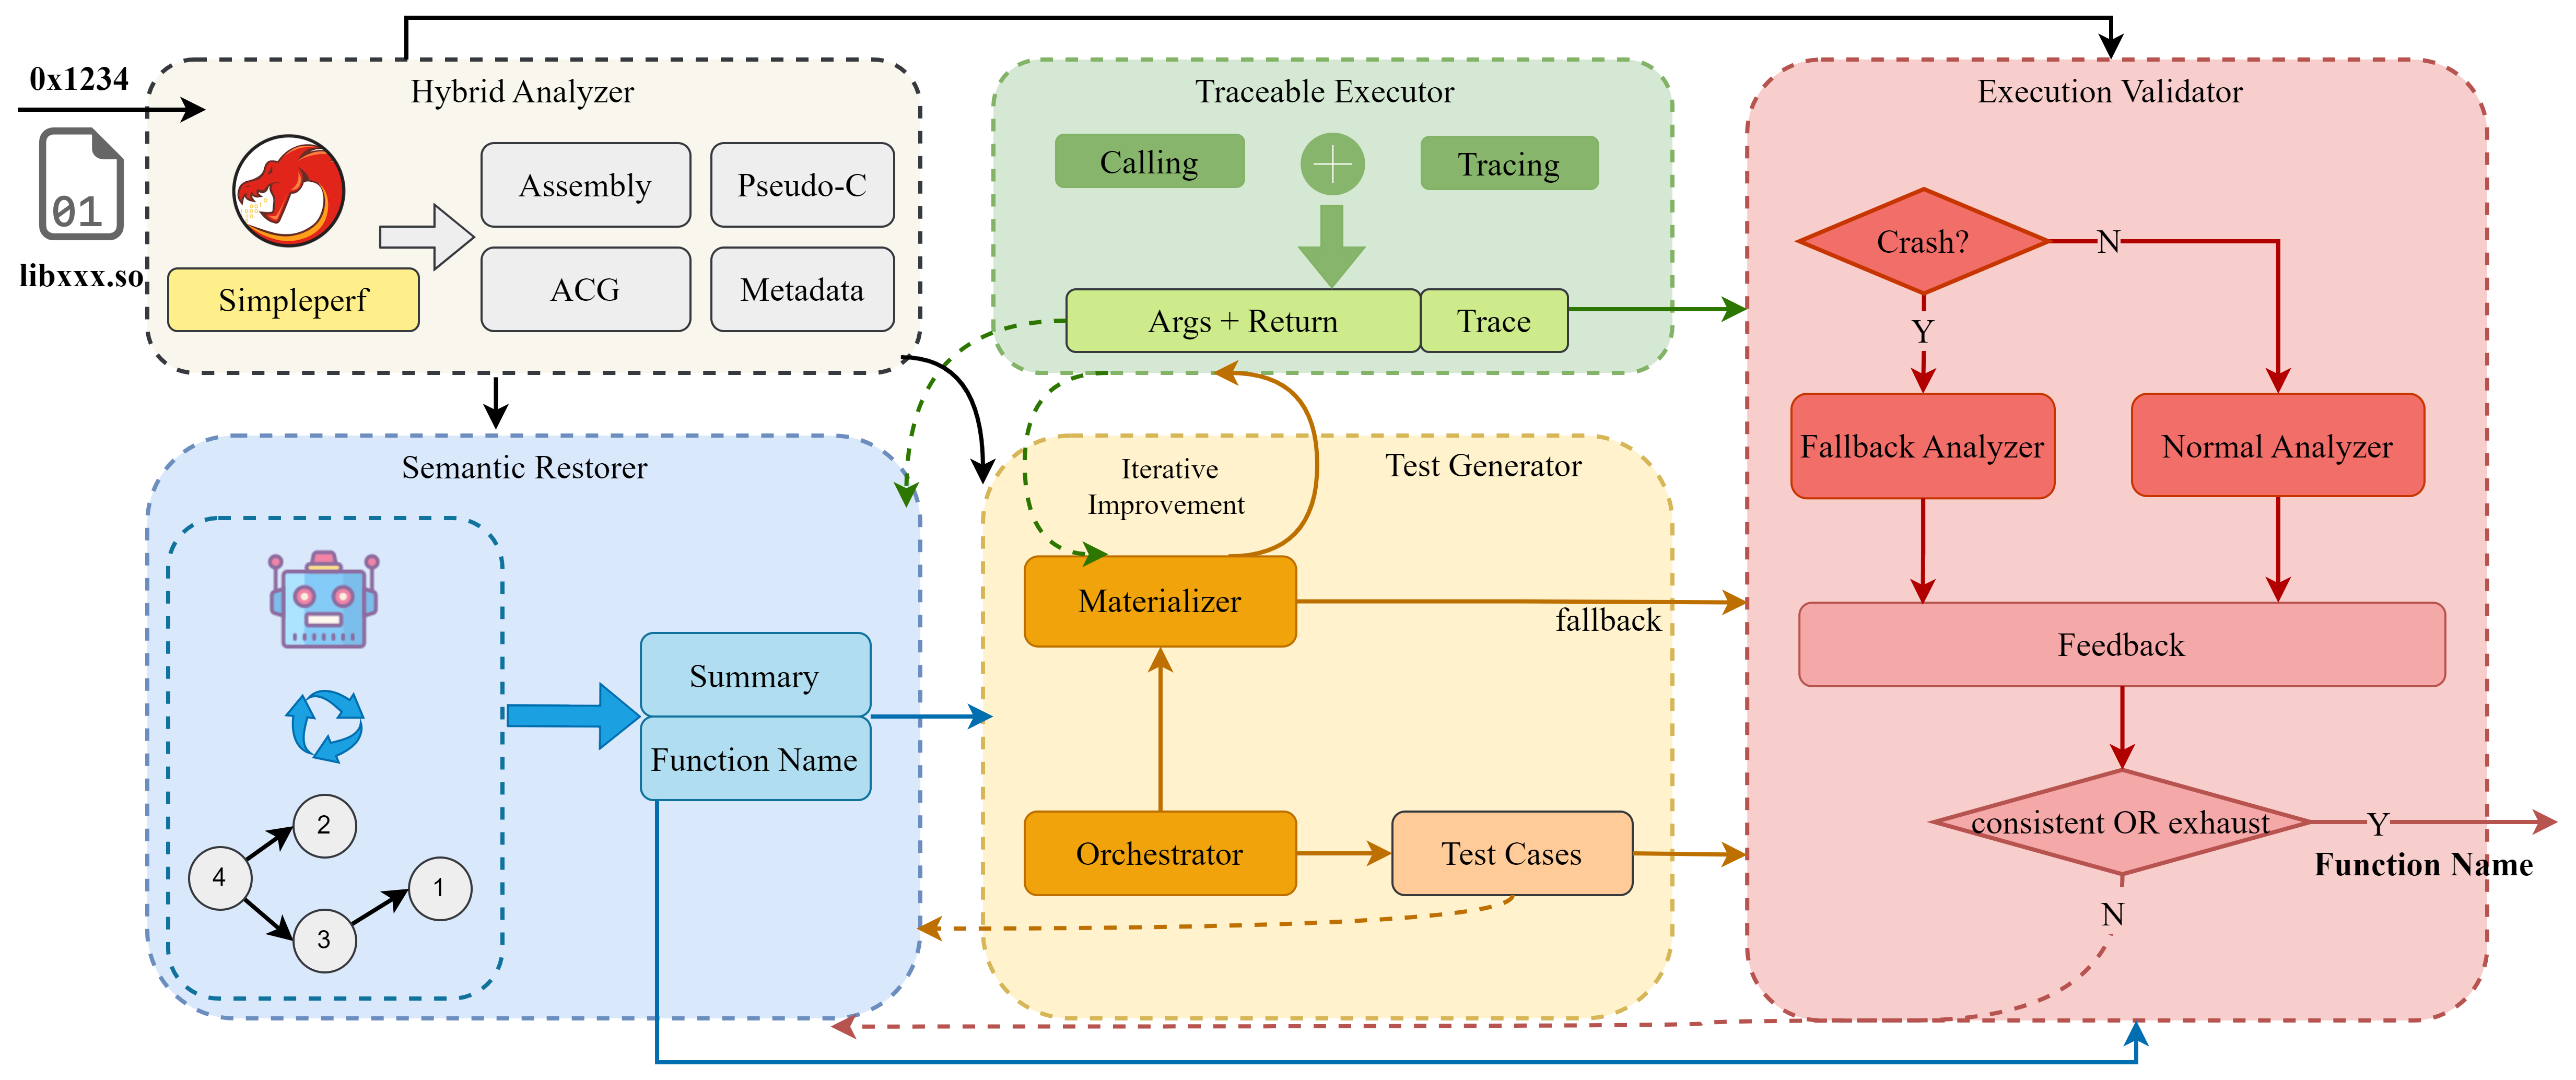
\includegraphics[width=0.5\textwidth]{image/Overview.drawio.png} % 调整图片宽度为文本宽度的50%
    \caption{An overview of the Multi-Agent system based on Frida and Ghidra} % 添加图片标题
    \label{fig:overview} % 设置图片标签,方便引用
\end{figure}
\begin{algorithm}
  \caption{HyBinMAS}
  \label{alg:HyBinMAS}
  \begin{algorithmic}[1]
    \REQUIRE $o$: The Offset of target function, $L$: The so file containing target function, $M$: The maximum iterations, $R$: The maximum retries for execution failure, $K$: The maximum numbers of test cases
    \ENSURE $N$: The predicted function name
    
    \STATE $\langle A, P, CG, metadata \rangle \gets \text{HSDA}(o, L)$
    \STATE $\langle N, S \rangle \gets \text{SR}(CG, o, A, P, M, \text{NULL})$
    \FOR{$m \gets 1$ \textbf{to} $M$}
        \STATE $T \gets \text{TG}(N, S, P, K)$
        \STATE $F \gets []$
        \FORALL{$t \in T$}
            \STATE $\langle err, args, ret, trace \rangle \gets \text{Executor}(t, R)$
            \IF{$err \ne \text{NULL}$}
                \STATE $f \gets \text{FallbackAnalyer}(t, err)$
            \ELSE
                \STATE $f \gets \text{NormalAnalyzer}(t, args, ret, trace)$
            \ENDIF
            \STATE $F.\text{push}(f)$
        \ENDFOR
        \STATE $feedback \gets \text{generate\_feedback}(F)$
        \IF{$\text{consistent\_check}(feedback)$}
            \RETURN $N$
        \ENDIF
        \STATE $\langle N, S \rangle \gets \text{SR}(CG, o, A, P, metadata, feedback)$
    \ENDFOR
    \RETURN $N$
  \end{algorithmic}
\end{algorithm}

The process is initiated by providing HyBinMAS with its inputs: the binary file, control parameters outlined in Algorithm \ref{alg:HyBinMAS}, and a target function uniquely identified by its offset. The process then unfolds as follows: \textbf{(\textit{i})} The \textbf{HSDA} performs a hybrid static-dynamic analysis on the target function and its containing binary file, yielding the function's assembly code, decompiled pseudo-code, call graph, and other pertinent metadata (Line 1 of Algorithm \ref{alg:HyBinMAS}). \textbf{(\textit{ii})} The \textbf{SR} leverages this comprehensive information to generate an initial predicted function name and a semantic summary (Line 2 of Algorithm \ref{alg:HyBinMAS}). \textbf{(\textit{iii})} Subsequently, the \textbf{TG} synthesizes a suite of suitable test cases based on the decompiled code from the HSDA and the name and summary provided by the SR (Line 4 of Algorithm \ref{alg:HyBinMAS}). \textbf{(\textit{iv})} The \textbf{Executor} then proceeds to run each test case generated by the TG, capturing both the execution traces and any error information. \textbf{(\textit{v})} Finally, the \textbf{EV} analyzes the outcome of each execution. Depending on whether a test case succeeded or failed, it selects an appropriate analyzer to process the results, summarize the collective execution feedback from the entire test suite and replay it to the SR for refinement and improvement.

As illustrated by Algorithm \ref{alg:HyBinMAS}, HyBinMAS performs at least one initial static analysis pass with the SR. This is followed by an iterative refinement loop (Lines 6-19), which repeats steps \textbf{(\textit{iii})}, \textbf{(\textit{iv})}, \textbf{(\textit{v})} and \textbf{(\textit{ii})} for up to $M$ iterations to progressively improve the initial semantic inference of SR. In the following sections, we will elaborate on the details of each step.


% Inspired by the typical workflow of human understanding of Android Native Functions, we have developed BinMAS, a Multi-Agent system based on tools such as Ghidra and Frida. BinMAS decomposes this workflow into five sub-tasks, each modeled and handled by a distinct Agent: the Static Information Agent (SIA), the Execution Agent (EA), the Semantic Analysis Agent (SAA), the Test Case Generation Agent (TCGA), and the Validation Agent (VA). To maximize the capabilities of each Agent and enhance the overall performance, we organize them according to the structure shown in \ref{fig:overview}. Herein, hollow and dashed arrows represent the data flow between different Agents, while solid arrows indicate data flow between components within the same Agent. Additionally, the components and their contents for each Agent are denoted by a consistent color scheme (e.g., EA is marked in green).

% For a target function, identified by its offset relative to the base address of the .so file, SIA is first employed to acquire its static information. This static information is then fed into the SAA as its primary input, prompting the corresponding LLM to generate semantic information about the function, including a proposed function name and summary. This semantic information, along with the static information from SIA, serves as input for the TCGA to construct corresponding test cases. Within the EA, we have established a Frida-based runtime environment for information acquisition. It accepts the test cases from TCGA and the basic information from SIA to execute the target function and capture its dynamic execution information (see Section xxx for details). The outputs from the preceding four Agents are all provided as part of the prompt to the VA. The VA's role is to validate the correctness of the semantic understanding produced by the SAA. If the understanding is deemed correct, it is accepted as the final result. Otherwise, the VA must provide detailed explanations and suggestions for revision. This feedback, along with the test cases and dynamic execution information, is passed back to the SAA for refinement. This process iterates until the VA's validation is successful or a predefined threshold is reached. In the following sections, we will discuss each agent in detail.

\subsection{Static Information Agent Design}

The SIA marks the starting point of the entire workflow. A target function (e.g., libnative-lib.so[+0x1234]) is first provided as input to the SIA. Here, BinMAS utilizes static analysis tools like Ghidra to analyze it, yielding disassembled code, decompiled C code, and metadata about the function (including its function signature, call graph, etc.). Consistent with prior research, BinMAS uses this static information as a basis for semantic inference. However, BinMAS goes a step further by integrating this static information with other sources, such as dynamic information, to jointly infer the semantics (see Section xxx for details).

\subsection{Semantic Analysis Agent Design}

The SAA is the core component of BinMAS. It is responsible for receiving the input from SIA and then querying an LLM for the semantic information of the target function, guided by our designed prompt templates. Notably, recognizing the inherent difficulty of binary semantic understanding (as opposed to source code analysis), we do not treat it as a single-turn process. Instead, we model it as a multi-turn, iterative refinement process. Therefore, for all subsequent rounds of analysis after the initial one, the SAA also receives feedback from the VA (as will be detailed in a later section). This feedback is combined with the information provided by SIA to form the prompt template. Under the guidance of this template, the LLM analyzes the semantics of the target binary function and generates a function summary and a corresponding function name. An example of a specific prompt template is shown in Figure 2.


\subsection{Execution Agent Design}

The Execution Agent (EA) represents a key innovation within the BinMAS framework. To the best of our knowledge, this work is the first in the domain of binary code semantic understanding to incorporate actual runtime behavior. Existing research on binary semantic understanding predominantly considers only static semantic information, lacking the capability to incorporate dynamic execution information (although SymLM considers execution behavior, it simulates dynamic actions using static call graph information, which is still fundamentally static in nature). This limitation arises because their target, stripped binaries, is overly broad, spanning multiple architectures and diverse application types, which makes it challenging to construct a unified execution environment. In contrast, BinMAS circumvents this issue by focusing on Android Native libraries, leveraging the inherent executability of apps to naturally construct a runtime environment.

Specifically, the EA leverages the powerful dynamic instrumentation tool, Frida, to intercept target functions. Frida can locate functions in two ways: by name or by offset address. Since many symbols are stripped in release builds of applications, we must rely on offset addresses to locate the target functions. This process is known as Frida hooking. Following the Frida hooking operation, we employ Stalker, a feature provided by Frida for instruction tracing, to capture the runtime behavior of the target function. We focus on two types of information: the function's runtime parameters, return value, and its execution trace.

\subsubsection{Acquiring Trace Information}

We construct the trace using CPU context information, specifically the state of the registers. This approach is chosen because the ARM64 architecture provides a significantly larger number of programmer-visible registers compared to the x86 architecture. As shown in Table~\ref{tab:arm_registers}, the ARM64 architecture offers 32 general-purpose registers and 32 vector registers. The general-purpose registers can act as units of different sizes (ie. 1B, 2B, 4B and 8B) depending on the operation type. The vector registers are even more versatile, supporting parallel computations in addition to using their lower 32 bits to represent \texttt{float} values and their lower 64 bits for \texttt{double} values. Furthermore, these registers are preferentially used for passing arguments and return values, as well as for storing temporary variables.

Since the execution of each instruction alters the context state, providing context at an instruction-level granularity is a trivial approach. However, given the large number of registers in the ARM64 architecture, providing the complete register state for every instruction would significantly exceed the context window of an LLM and could also induce hallucinations. Therefore, we implemented the following optimizations:
\begin{enumerate}
    \item \textbf{Minimize Register Information:} We select all general-purpose registers. For vector registers, we only consider common access patterns, namely as \texttt{float} and \texttt{double} values.
    \item \textbf{Differential Tracing:} We provide the complete register state only at the function's entry and exit points. For each intermediate instruction, we only report the registers that have changed relative to the previous step. Subsequent experiments demonstrate that this approach helps the model focus on the semantics of individual instructions, thereby improving the overall accuracy of semantic understanding.
\end{enumerate}

\subsubsection{Acquiring Parameters and Return Values}

Although the standard calling convention in the ARM64 architecture dictates that parameters and return values are passed via registers, which implies that, in most cases, this information would already be captured within the execution trace, we find it beneficial to handle them explicitly. Because parameter and return value information is highly indicative of a function's semantics, highlighting it can significantly aid the LLM in its semantic comprehension. To this end, we leverage Ghidra's static analysis capabilities to precisely identify these values. This process also enables the discovery of parameters stored on the stack.



\subsection{Test Case Generation Agent Design}

We reiterate that relying solely on static information for semantic understanding by the SAA is often insufficient, as this approach would effectively regress to those of prior studies (i.e., leveraging LLMs to understand decompiled code). Our key insight is that runtime information accurately reflects a program's execution state, making it an inherent basis for validation. To acquire this runtime information, we need appropriate test cases to trigger the relevant program behaviors. Ideally, such test cases should compensate for the inaccuracies and ambiguities present in static information. While established techniques for test case generation exist, such as fuzzing and symbolic execution, they often lack the ability to intelligently select context-aware inputs. Recent studies have demonstrated the significant potential of LLMs for test case generation. Consequently, BinMAS leverages this capability as the core foundation of the Test Case Generation Agent (TCGA).

In BinMAS, the prompt template used for generating test cases with an LLM is detailed in Section~xxx. An example of the generated output is also provided.

\subsection{Validation Agent Design}

The rationale for designing the Validation Agent (VA) stems from a fundamental limitation of dynamic analysis: a single execution trace, while concrete, does not guarantee full path coverage. This means that a single run is unlikely to exercise all execution paths, potentially omitting critical logic. To address this, BinMAS employs the VA to validate the semantic understanding produced by the SAA. If the validation is successful, it is concluded that the SAA's output accurately reflects the logic of the target function. Conversely, if validation fails, the SAA's output is considered discrepant. The VA then provides a detailed explanation and suggestions for revision. This feedback, along with the test case and execution trace, is passed back to the SAA to guide the next iteration of analysis.

Evidently, the outcome of the VA's validation critically influences the number of iterations in the workflow and, in turn, affects the overall efficacy of our method. To minimize the potential for error in the VA's judgment, we furnish it with a rich set of contextual information. As depicted in Figure~xxx, the function metadata from SIA is included as part of the VA's prompt template. The test case generated by the TCGA is another essential component, and the execution trace obtained by the EA is also supplied as input. The output from the SAA serves as the object of validation. Furthermore, we incorporate specific instructions in the prompt to guide the model to produce output in a structured format (e.g., a pass/fail decision, the rationale for failure, etc.).



\section{Implementation and Evaluation}

\subsection{Dataset}
\begin{figure}[h] % [h] 表示图片放置在当前位置
    \centering
    \includegraphics[width=0.5\textwidth]{image/ConstructDataset.drawio.png} % 调整图片宽度为文本宽度的50%
    \caption{An overview of the dataset construction process} % 添加图片标题
    \label{fig:construct-dataset} % 设置图片标签,方便引用
\end{figure}

To the best of our knowledge, no dedicated dataset currently exists for semantic understanding tasks on Android Native Libraries, such as function name recovery and comment generation. Although numerous data sets are available for stripped binaries,ies, they are inadequate for our purposes. These existing datasets either lack compilation variants for the ARM64 architecture or are not executable on Android devices, which is unacceptable for our method. Therefore, we are working on the construction of a new specialized dataset. The overview of this process is illustrated in Figure 3.

\textbf{1)Android Project Selection}. Our ultimate objective is to analyze closed-source applications. Therefore, the primary principle guiding our selection of open-source projects is to ensure they accurately reflect the characteristics of their closed-source counterparts. Inspired by BinMetric and BinaryLLM-Eval, we adapt and extend their critera to align with the specific requirements of our work:

\begin{itemize}
    \item \textbf{Executability:} The requirement for executability is twofold. The first consideration is practical applicability, necessitating that the target application be runnable. The second is the operational constraints imposed by the EA within our proposed approach.
    
    \item \textbf{Native Code  Availability:} Selected projects must contain native source code (implemented in C or C++). This is crucial as projects providing only pre-compiled .so files would prevent us from obtaining the ground-truth function semantics (i.e., names and comments). It is critical that the target functions must be non-exported. This ensures that their symbol information can be completely removed during the stripping process without impairing the application's runtime functionality—a task that is infeasible for exported functions.

    \item \textbf{Realisticity and Modernity:} To ensure the dataset reflects contemporary, real-world scenarios, the selected projects must be compatible with latest Android versions. At the time of our data collection, with Android 14+ gradually becoming the mainstream system, we established Android 15 compatibility as our target standard.

    \item \textbf{Project Quality:} High-quality projects are essential, as factors like code clarity and structure can significantly influence the performance of semantic analysis. We identified quality through characteristics such as a well-organized project structure, clear logical implementation, and adherence to good naming conventions. Project quality can be quantifiedby its Stars and Forks on GitHub.

    \item \textbf{Domain Diversity:} To comprehensively evaluate the generalization capabilities of our proposed method, the dataset should encompass applications from a broad range of domains. We identified and included projects from the following categories: Communication \& Social Networking,  Science \& Education, Multimedia, Game, Finance and Tools. It is important to acknowledge that these categories do not cover the full spectrum of real-world applications. Numerous projects from other domains were filtered out as their failure to meet the 1st criterion.

    \item \textbf{Maintenance Status:} To ensure the relevance of the compiled binaries and their underlying code, projects were required to have a recent history of updates or maintenance. We have chosen 5 years as the threshold.
\end{itemize}

From an initial survey of [Number] Android application projects, we downloaded [Number] candidates based on the requirements outlined above. During the subsequent compilation and build process, we filtered out any project that could not be constructed as specified (see details below), resulting in a final corpus of [Number] APKs. These artifacts are then subjected to the subsequent processing stages (Steps \normalsize{\textcircled{\scriptsize{3}}}\normalsize–\normalsize{\textcircled{\scriptsize{7}}}\normalsize) illustrated in Figure 3.


\textbf{2)APK Construction}. We utilized Gradle to complete the build tasks. For each application, we compiled two distinct variants: **Release** and **Release-DWARF**. It is important to note that we deliberately avoided the common practice of building a standard Debug version with DWARF information for its Release counterpart. This is because build tools like Gradle and the NDK apply different configurations (e.g., varying optimization levels) to Debug and Release builds. Such discrepancies will result in non-identical native code, thereby complicating the subsequent alignment process.

Instead, our approach uses the standard Release as the baseline. We generate the **Release-DWARF** variant by augmenting the Release binaries with DWARF information while ensuring the underlying machine code remained unchanged. The final executable deployed on the Android system is also the standard Release, which perfectly aligns with real-world scenarios. Consistent with established practices in previous research, we apply Step \normalsize{\textcircled{\scriptsize{3}}}\normalsize, employing Ghidra to generate the corresponding disassembly and pseudo-C code for these binaries.


\textbf{3)Ground-Truth Construction}. This process begins with the extraction of native source code from the selected projects (as shown in step \normalsize{\textcircled{\scriptsize{4}}}\normalsize).
\begin{itemize}
    \item For the \textbf{Function Name Recovery (FNR)} task, we designated the developer-written function names as the ground-truth. This was accomplished by parsing the C/C++ source code using tree-sitter (\normalsize{\textcircled{\scriptsize{6}}}\normalsize).
    \item For the \textbf{Binary Summarization} task, we opted \textbf{NOT} to use the comments present in the source code. As demonstrated by previous research, these comments often suffer from low quality and incompletion. Conversely, a significant body of work has demonstrated that LLMs, exemplified by GPT, can generate high-quality, descriptive summaries—often surpassing the quality of those written by human developers. Therefore, we employed an LLM to perform this summarization task (\normalsize{\textcircled{\scriptsize{5}}}\normalsize).
\end{itemize}


\textbf{4)Alignment}. In step \circlenum{2}, we obtained the binary variant that includes DWARF information. This variant shares identical function address offsets with its stripped counterpart, which allows for a straightforward alignment of the function body with their corresponding function name. Furthermore, the DWARF data contains precise records of the source code locations (i.e., file and line number) for each function and variable. This information serves as the definitive basis for aligning the decompiled pseudo-C code with the original source code. Through this two-step alignment process, we can reliably link each function in the binary (represented by both its assembly and pseudo-C code) to its corresponding ground-truth.


\textbf{5)Filtering and Leakage Check}. To accurately simulate the senarios of real-world applications, we implemented two filtering steps. First, we filtered out any functions that retained their symbol information post-stripping to avoid overestimating the method's performance. Second, we discarded functions with very small bodies (defined as having fewer than 5 assembly instructions).

Performing a data leakage check on the pseudo-C code within our dataset is a crucial final step. This is to ensure that the data has not been seen by the LLM during its pre-training phase. Following the methodology of existing research in related fields, we conducted this check by tasking an LLM with a pseudo-C code completion challenge. We observed that the average similarity between the LLM's auto-completed code and the original pseudo-C code was merely xxx-. This low score indicates that our dataset successfully passes the leakage check, confirming its novelty and suitability for training and evaluation.

Ultimately, we get xxx Android projects for our dataset. Detailed information for each project is presented in Table 1.



\subsection{Research Questions}



\section{Threats to Validity}




\section{Related Work}
\subsection{Symbol Recovery}

The strip command, a standard utility in toolchains, removes symbol information from binaries, including variable names and type definitions. The absence of this information significantly impedes the comprehension and analysis of binaries. Consequently, a substantial body of research has been dedicated to recovering these symbols. Despite pioneering efforts in this domain (Debin, DIRE, NERO, NFRE, Punstrip, and DIRTY), further research is needed to advance the symbol recovery task.

One major line of research focuses on the recovery of variables and data structures, such as (TypeFSL, ReSym, HyRES, TypeForge). Another significant research direction, which aligns with one of the primary goals of this paper, is the recovery of function names. Meaningful function names provide a global summary of a subroutine's purpose, making them invaluable for program understanding. Recent works such as SymLM and ASMDepictor have leveraged the powerful encoding capabilities of Transformers to convert assembly code into semantic embeddings for predicting function names. To address the practical challenge of out-of-vocabulary (OOV) function names, XFL models the task as a multi-label classification problem, predicting each sub-token of a function name individually. More innovatively, SymGen reformulates function name recovery as a generative task and trains a bespoke LLM for this purpose. This approach effectively resolves the poor generalization caused by the OOV problem in previous methods and achieves results that significantly surpass prior work.

While our methodology shares conceptual similarities with Sym-LM's use of dynamic analysis, our approach orchestrates a Multi-Agent system for collaborative reasoning and inference, allowing for a more effective use of dynamic information.

\subsection{Code Summarization}
\textbf{Code Summarization}, the task of generating concise natural language descriptions for a given piece of code, is indispensable for program comprehension. The field has primarily focused on source code summarization, for which a wide array of techniques have been developed. These methodologies have evolved from early template-based and information retrieval (IR) approaches to more sophisticated techniques grounded in deep learning. Most recently, the advent of Large Language Models (LLMs) has marked a paradigm shift. LLM-based methods are now considered the state-of-the-art, with studies showing their generated summaries can sometimes even surpass the quality of human-written reference comments.

However, a considerable semantic gap persists when applying LLMs to binary code, as these models often struggle to understand low-level machine instructions without symbolic information. Although some researchers have begun to explore LLM-based binary code summarization, as exemplified by work such as FoC, these pioneering efforts predominantly rely on fine-tuning bespoke models for this specific task. Inspired by the remarkable performance of Multi-Agent systems in solving complex reasoning tasks in other domains, our method leverages a Multi-Agent system to collaboratively guide and enhance an LLM's comprehension and reasoning capabilities over binary code.


\subsection{LLM for Binaries}
LLMs have demonstrated remarkable success across a spectrum of source code-related tasks (). As LLM technology continues to evolve, a growing body of research has started to explore its application in the binary analysis domain, including symbol recovery (e.g., ReSym, HyRES, SymGen) and the improvement of decompilation output (e.g., LLM4Decompile, DeGPT).

However, for practitioners in the field, such as reverse engineers, a more fundamental challenge lies in the semantic comprehension of the binary code itself. FoC begins to address this critical need, but its approach has two significant limitations: its applicability is confined to the specific domain of cryptographic functions, and it necessitates the fine-tuning of a dedicated LLM. In stark contrast, our method is designed to be domain-agnostic, imposing no restrictions on the type of binary, and obviating the significant computational and data overhead associated with model training.



\section{Conclusion}




%%
%% The acknowledgments section is defined using the "acks" environment
%% (and NOT an unnumbered section). This ensures the proper
%% identification of the section in the article metadata, and the
%% consistent spelling of the heading.
\begin{acks}
To Robert, for the bagels and explaining CMYK and color spaces.
\end{acks}

%%
%% The next two lines define the bibliography style to be used, and
%% the bibliography file.
\bibliographystyle{ACM-Reference-Format}
\bibliography{sample-base}


%%
%% If your work has an appendix, this is the place to put it.
\appendix

% \section{Research Methods}

% \subsection{Part One}

% Lorem ipsum dolor sit amet, consectetur adipiscing elit. Morbi
% malesuada, quam in pulvinar varius, metus nunc fermentum urna, id
% sollicitudin purus odio sit amet enim. Aliquam ullamcorper eu ipsum
% vel mollis. Curabitur quis dictum nisl. Phasellus vel semper risus, et
% lacinia dolor. Integer ultricies commodo sem nec semper.

% \subsection{Part Two}

% Etiam commodo feugiat nisl pulvinar pellentesque. Etiam auctor sodales
% ligula, non varius nibh pulvinar semper. Suspendisse nec lectus non
% ipsum convallis congue hendrerit vitae sapien. Donec at laoreet
% eros. Vivamus non purus placerat, scelerisque diam eu, cursus
% ante. Etiam aliquam tortor auctor efficitur mattis.

% \section{Online Resources}

% Nam id fermentum dui. Suspendisse sagittis tortor a nulla mollis, in
% pulvinar ex pretium. Sed interdum orci quis metus euismod, et sagittis
% enim maximus. Vestibulum gravida massa ut felis suscipit
% congue. Quisque mattis elit a risus ultrices commodo venenatis eget
% dui. Etiam sagittis eleifend elementum.

% Nam interdum magna at lectus dignissim, ac dignissim lorem
% rhoncus. Maecenas eu arcu ac neque placerat aliquam. Nunc pulvinar
% massa et mattis lacinia.

\end{document}
\endinput
%%
%% End of file `sample-sigconf-authordraft.tex'.
